\documentclass[a4paper,12pt]{article}


\usepackage[utf8]{inputenc}
%\usepackage{fullpage,color}
\usepackage{graphicx}
\graphicspath{ {./images/} }

\usepackage{amsthm}
\usepackage{amsfonts}
\usepackage{amsmath,amssymb}
\usepackage{mathtools}
\usepackage{physics}
\usepackage{comment,float}
\usepackage{filecontents}
\usepackage{pgfplots}
\usepgfplotslibrary{groupplots}
%\usepackage{glossaries}

\usepackage[ruled,vlined]{algorithm2e}

\usepackage{hyperref}
\hypersetup{
    colorlinks=true,
    linkcolor=blue,
    filecolor=magenta,      
    urlcolor=cyan,
}



\newtheorem{fact}{Fact}
\newcommand{\OPT}{\texttt{OPT}}
%\newcommand{\ball}{\text{ball}}

\newcommand{\I}{\mathbb{I}}
\newcommand{\Sim}{\mathcal{S}}
\newcommand{\Dis}{\mathcal{D}}
\newcommand{\cost}{\mathrm{cost}}
\newcommand{\N}{\mathbb{N}}
\newcommand{\R}{\mathbb{R}}
\newcommand{\V}{\mathbb{V}}
\newcommand{\C}{\mathcal{C}}
\newcommand{\net}{\mathcal{N}}
\newcommand{\mylabel}{\mathsf{label}}
\newcommand{\NN}{\mathsf{NN}}
\newcommand{\Lip}{\mathsf{Lip}}
\newcommand{\Int}{\mathsf{Int}}
\newcommand{\Vol}{\mathsf{Vol}}
\newcommand{\diam}{\mathsf{diam}}
\newcommand{\rad}{\mathsf{rad}}
\newcommand{\ball}{\mathsf{ball}}
\newcommand{\corruption}{\mathsf{corruption}}
\newcommand{\eps}{\varepsilon}

\newcommand{\Alg}{\textsf{Alg}}
\newcommand{\AlgKNNFlip}{\textsf{Poison-$k$-NN}}
\newcommand{\AlgOneMean}{\textsf{Poison-$1$-Mean}}
\newcommand{\AlgAntiG}{\textsf{Anti-Gonzalez}}
\newcommand{\AlgApproxEmptyBall}{\textsf{ApproxEmptyBall}}

\newcommand{\gls}[1]{\textbf{#1}}
\newcommand{\XXX}{\textcolor{red}{XXX}}
\newcommand{\TODO}{\textcolor{red}{TODO:}}
\newcommand{\WIP}{\textcolor{green}{WIP}}

\DeclareMathOperator*{\argmax}{arg\,max}
\DeclareMathOperator*{\argmin}{arg\,min}
\DeclareMathOperator*{\spann}{span}
%\DeclarePairedDelimiter{\abs}{\lvert}{\rvert}
%\DeclarePairedDelimiterX{\norm}[1]{\lVert}{\rVert}{#1}
\newcommand{\CC}[1]{\textcolor{red}{c_{#1}}}







\title{Poison-1-Mean Experiments}


\begin{document}

\maketitle


\begin{abstract}
We conduct experiments from the study that was performed on poisoning a geometric data sets.
In the research paper Algorithms for Poisoning Geometric Data Sets, we have an algorithm for
poisoning 1 mean clustering. This paper will run analysis on iris data, diabetes data and random
generated data. All of theses experiments are conducted in $\R^2$ Euclidean space
\end{abstract}

\section{Poisoning $1$-Mean Clustering}
\label{sec:1-mean}

In the $k$-means clustering problem, the input consists of a set of points, $X=\{1,\dots,x_n\}\subset [0,1]^d$, and the goal is to find a set of means, $M=\{\mu_1,\dots, \mu_k\}\subset [0,1]^d$, such that $\cost_k(X,M)=\sum_{x\in X}\min_{\mu\in M}\norm{x-\mu}^2_2$ is minimised. We use $\cost_k(X)$ to denote the optimal cost of $k$-means on $X$; that is
$\cost_k(X)=\inf_{M} \cost_K(X,M)$.
We refer to a set $\{\mu_1,\dots,\mu_k\}$ that minimizes $\cost(X)$ as \emph{optimal means}. We can define a function $\mu:X\to M$ as $\mu(x)=\argmin_{\mu\in M}\norm{\mu-x}_2$ where the ties are broken arbitrarily. The function $\mu$ then defines a partition $\{X_1,\dots,X_k\}$ of $X$ by setting $X_i:=\mu^{-1}(\mu_i)$.

The $m$-poisoning of $k$-means seeks a poison multiset $P=\{p_1,\dots,p_m\}\subset[0,1]^d$ such that $\cost_k(X\cup P)$ is maximized.

\textbf{Algorithm \AlgOneMean~for $1$-Mean Poisoning:}
The input consists of 
$n,m\in \mathbb{N}$,
and a set of points $X=\{x_1,\dots,x_n\}\subset [0,1]^d$,
with $|X|=n$.
The output is a poison $P=\{p_1,\dots,p_m\}\subset [0,1]^d$.
\begin{description}
    \item{\textbf{Step 1.}} 
    Let
    %Compute the $1$-mean, $\mu$, of $X$; that is
    \begin{align*}
        \mu = \frac{1}{n}\sum_{i=1}^n x_i
    \end{align*}
    \item{\textbf{Step 2.}} Find $p^*=\argmax_{p\in [0,1]^d}\norm{p-\mu}_2$
    \item{\textbf{Step 3.}}
    Let $P_\Alg$ be the multiset containing $m$ copies of $p^*$.
    Return $P_\Alg$.
%    Set $p_i\gets p^*$ for all $1\le i\le m$.
%    \item Return $\{p_1,\dots,p_m\}$
\end{description}
This concludes the description of the algorithm.
\\

\section{Random Data Experiment}
The random data experiment consisted of a bounding box with $p_1 = (0,0)$ and $p_2 = (1,1)$ \\
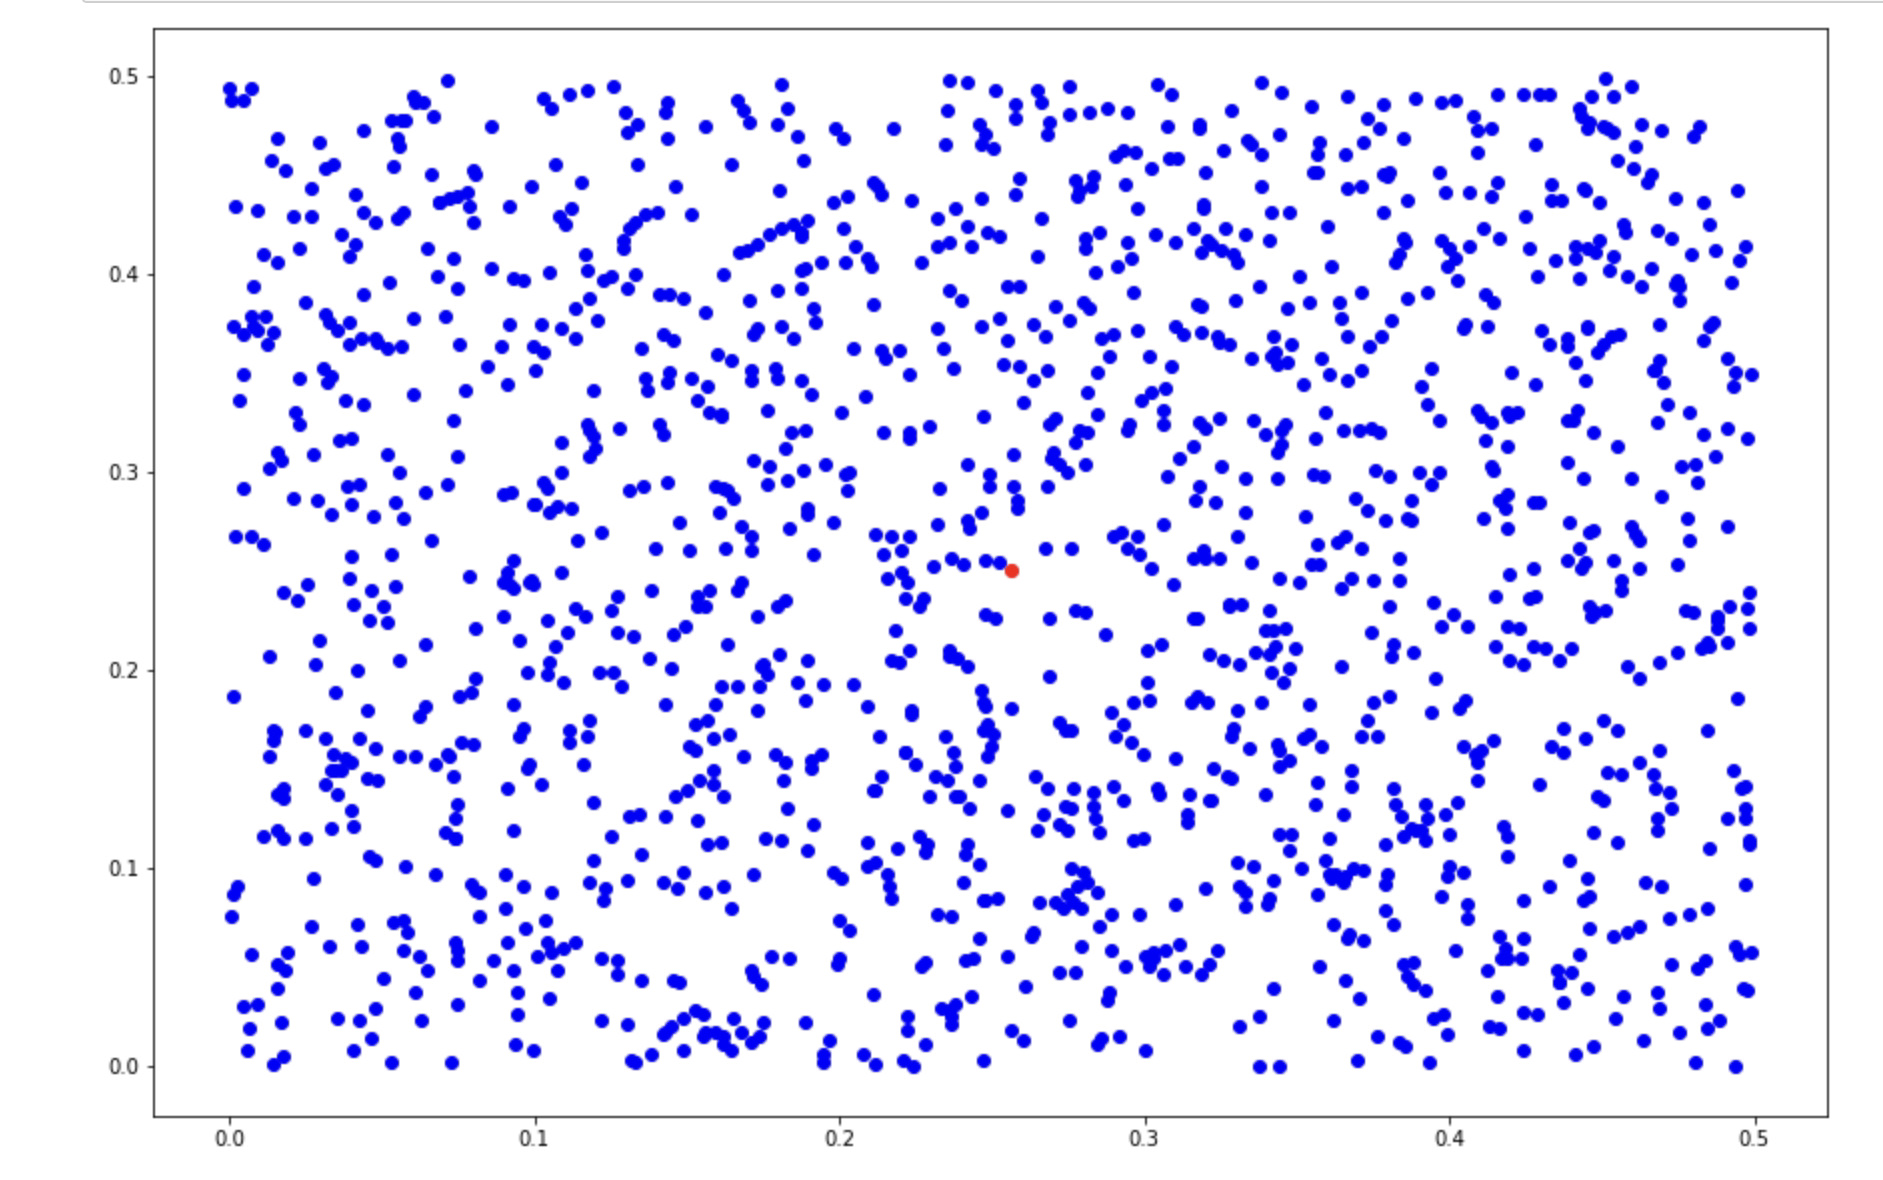
\includegraphics [width=5cm, height=4cm]{random_data}
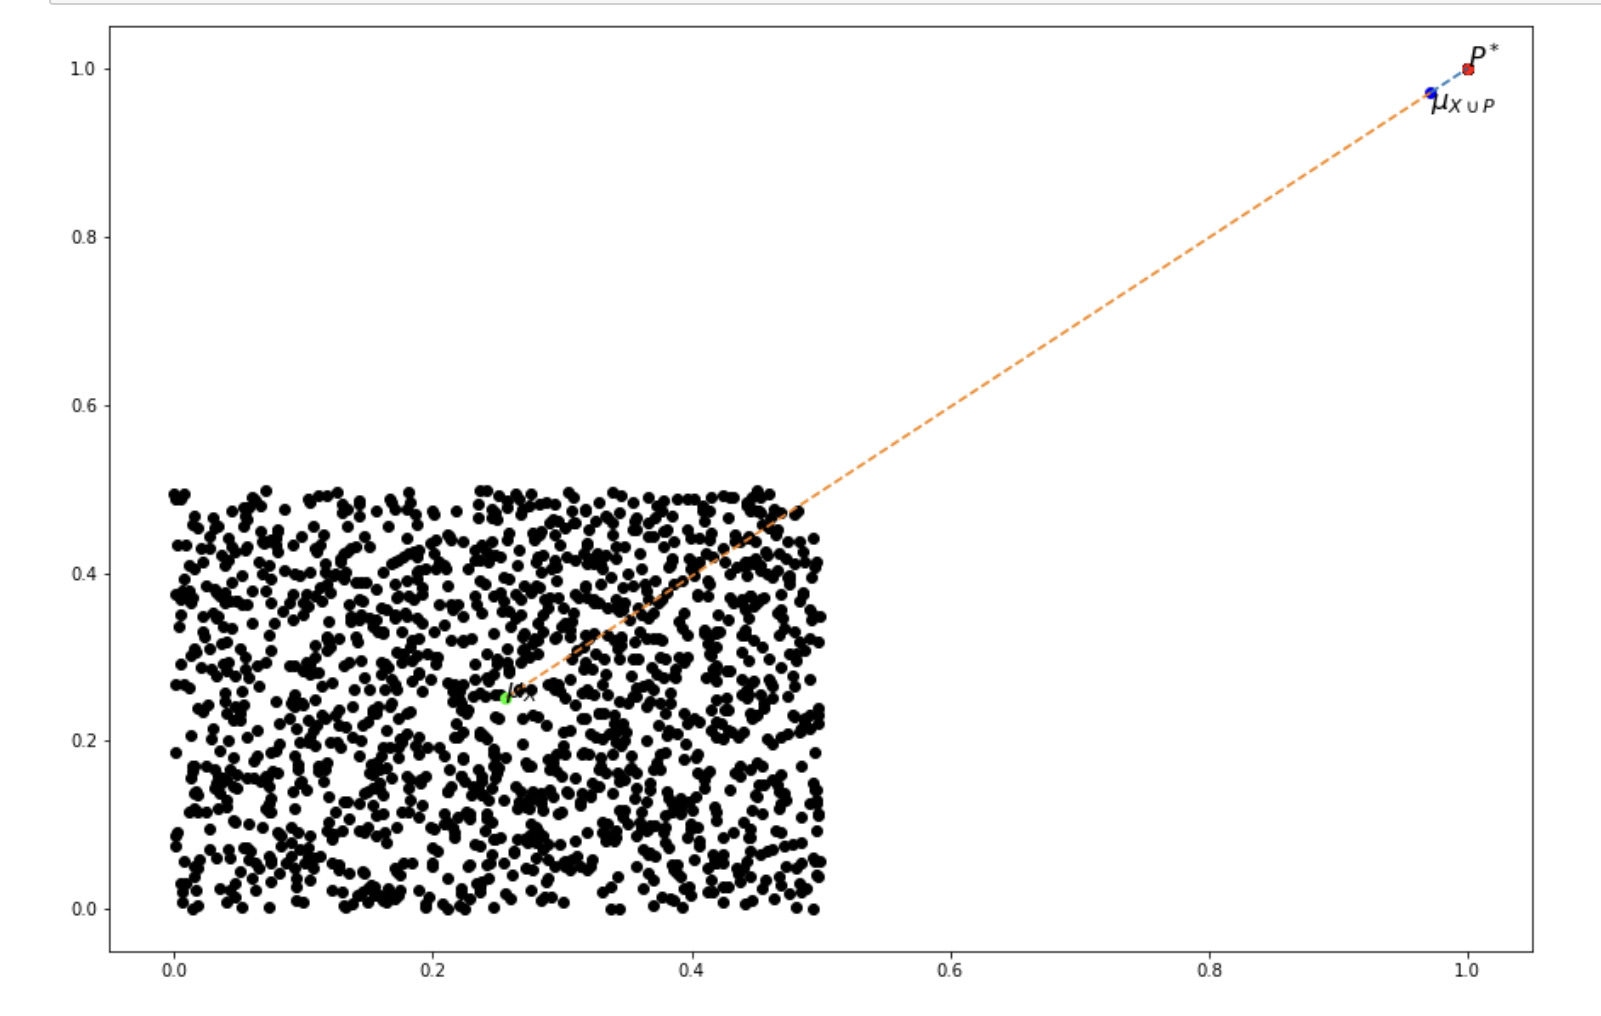
\includegraphics [width=5cm, height=4cm]{random_data_poisoned}
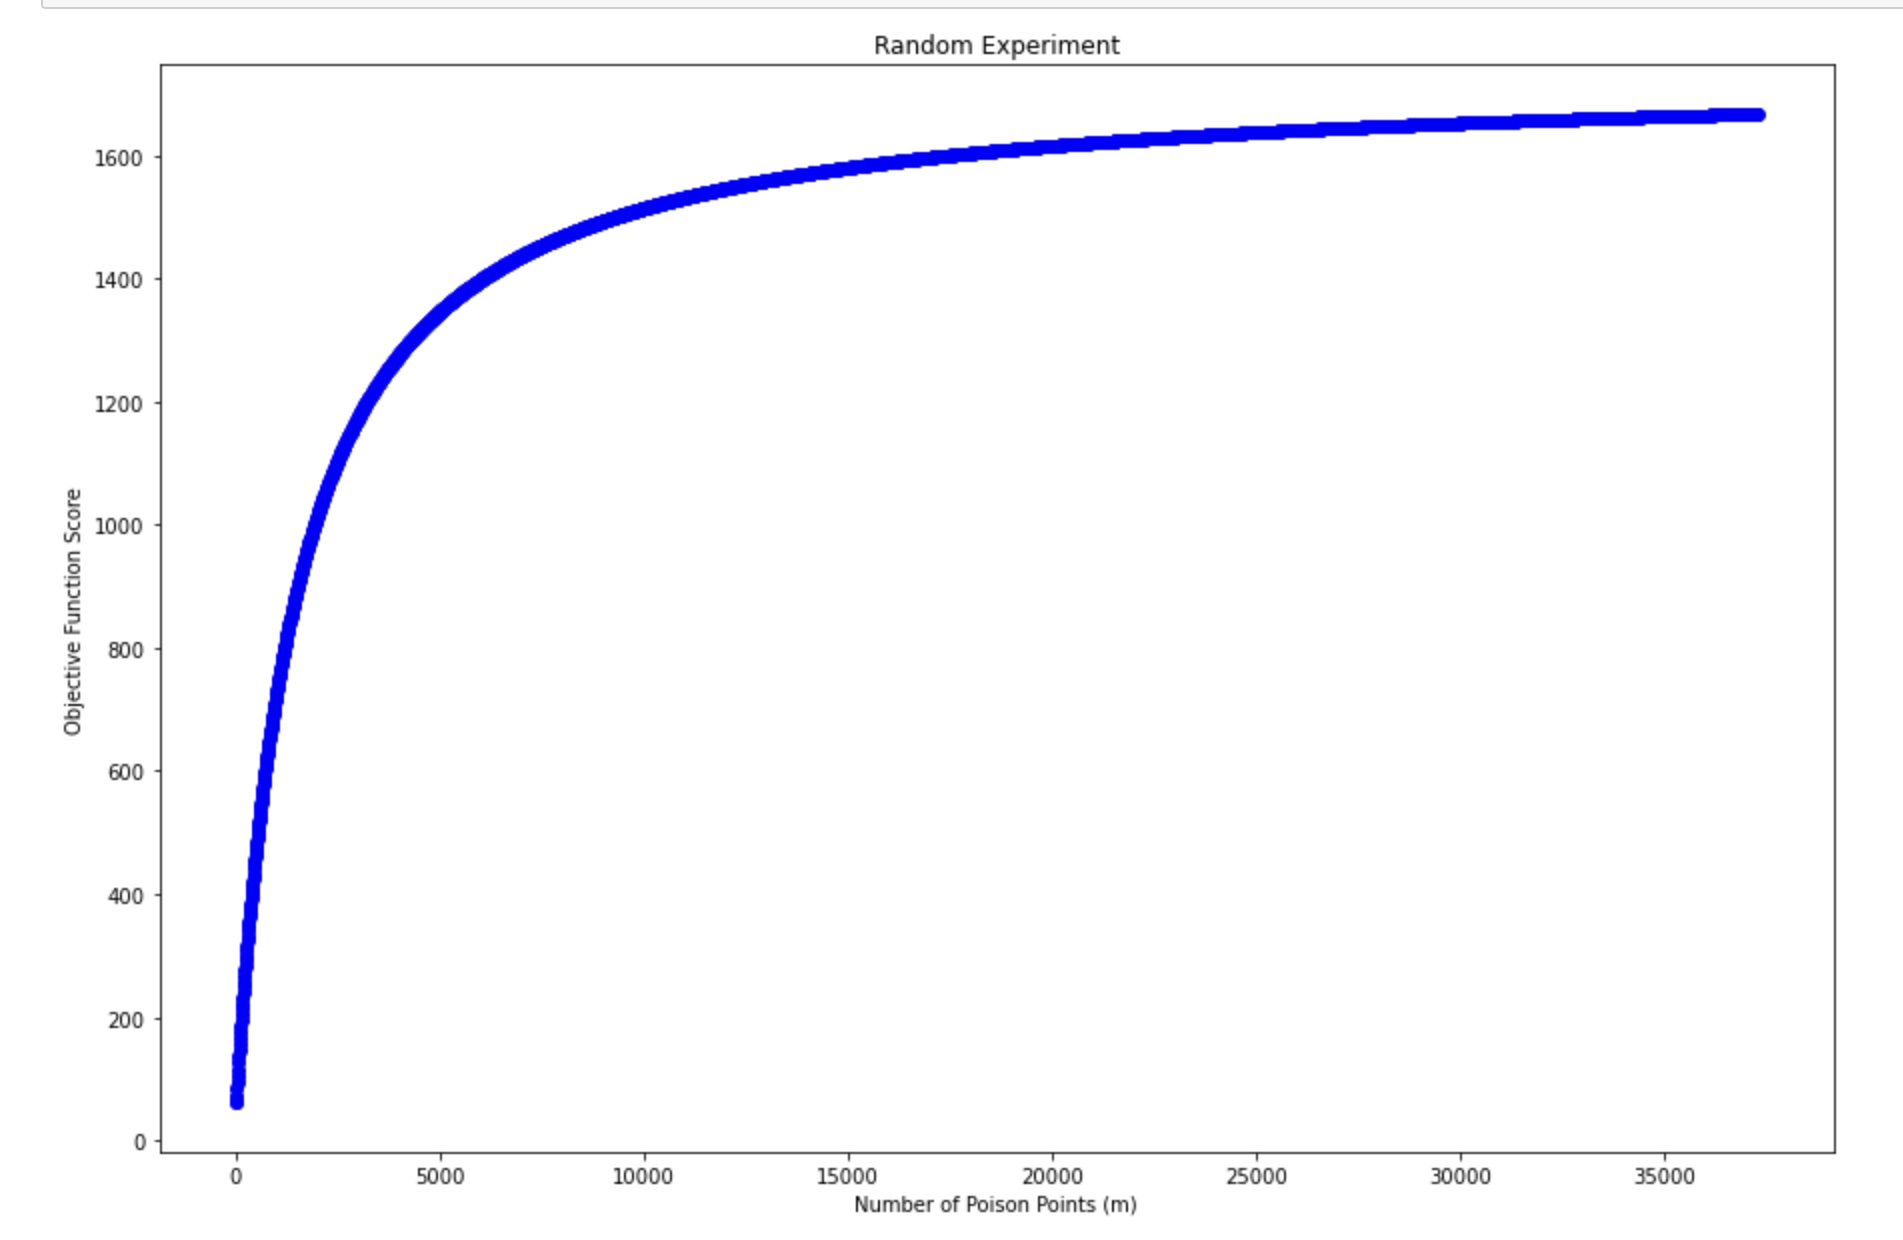
\includegraphics [width=5cm, height=4cm]{random_poison_vs_score}

\section{Iris Data Experiment}
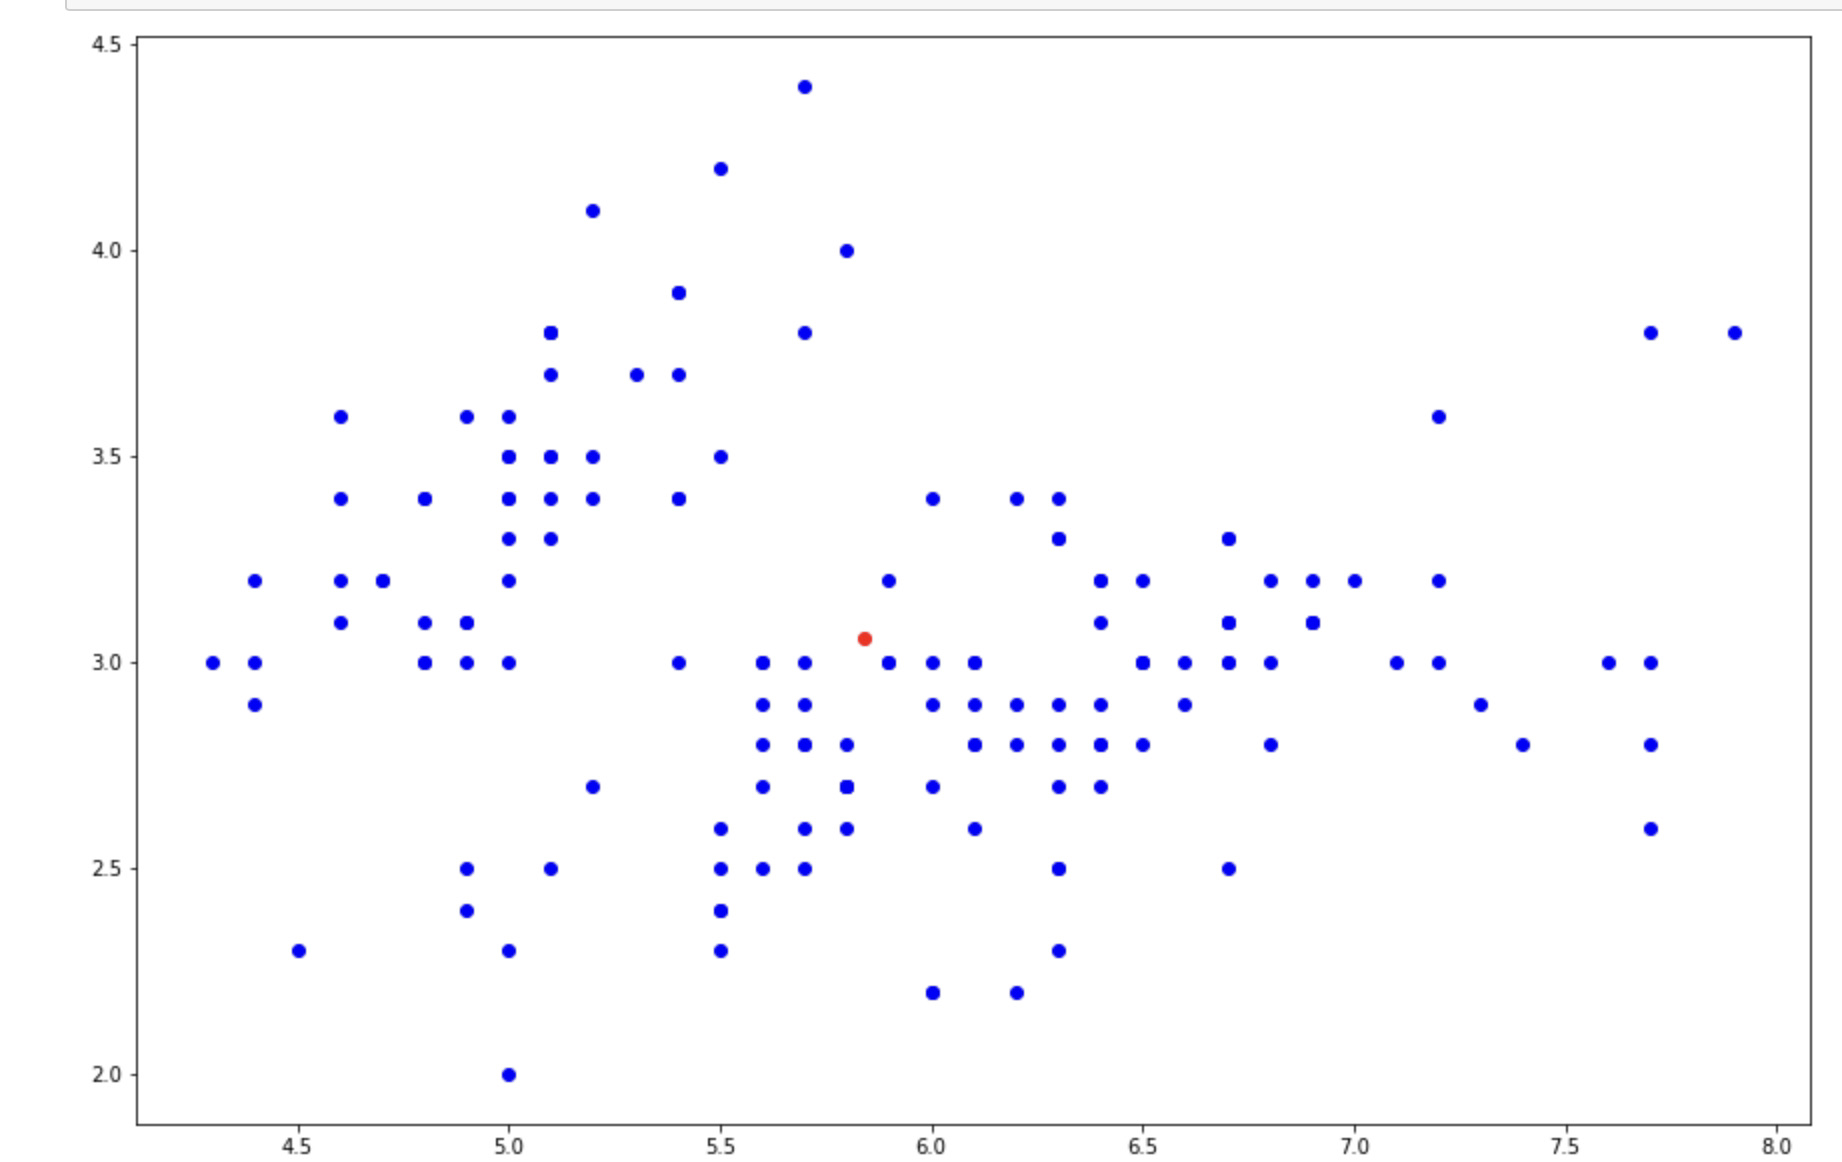
\includegraphics [width=5cm, height=4cm]{iris_data}
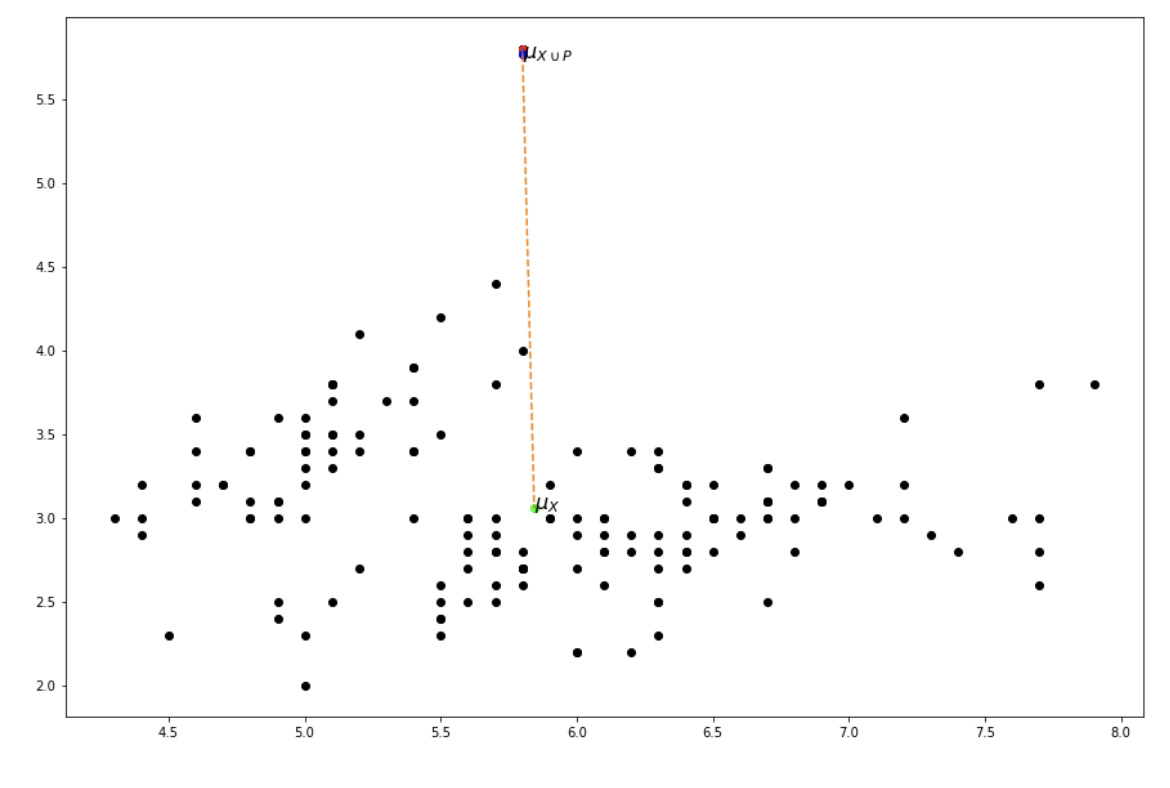
\includegraphics [width=5cm, height=4cm]{iris_data_poisoned}
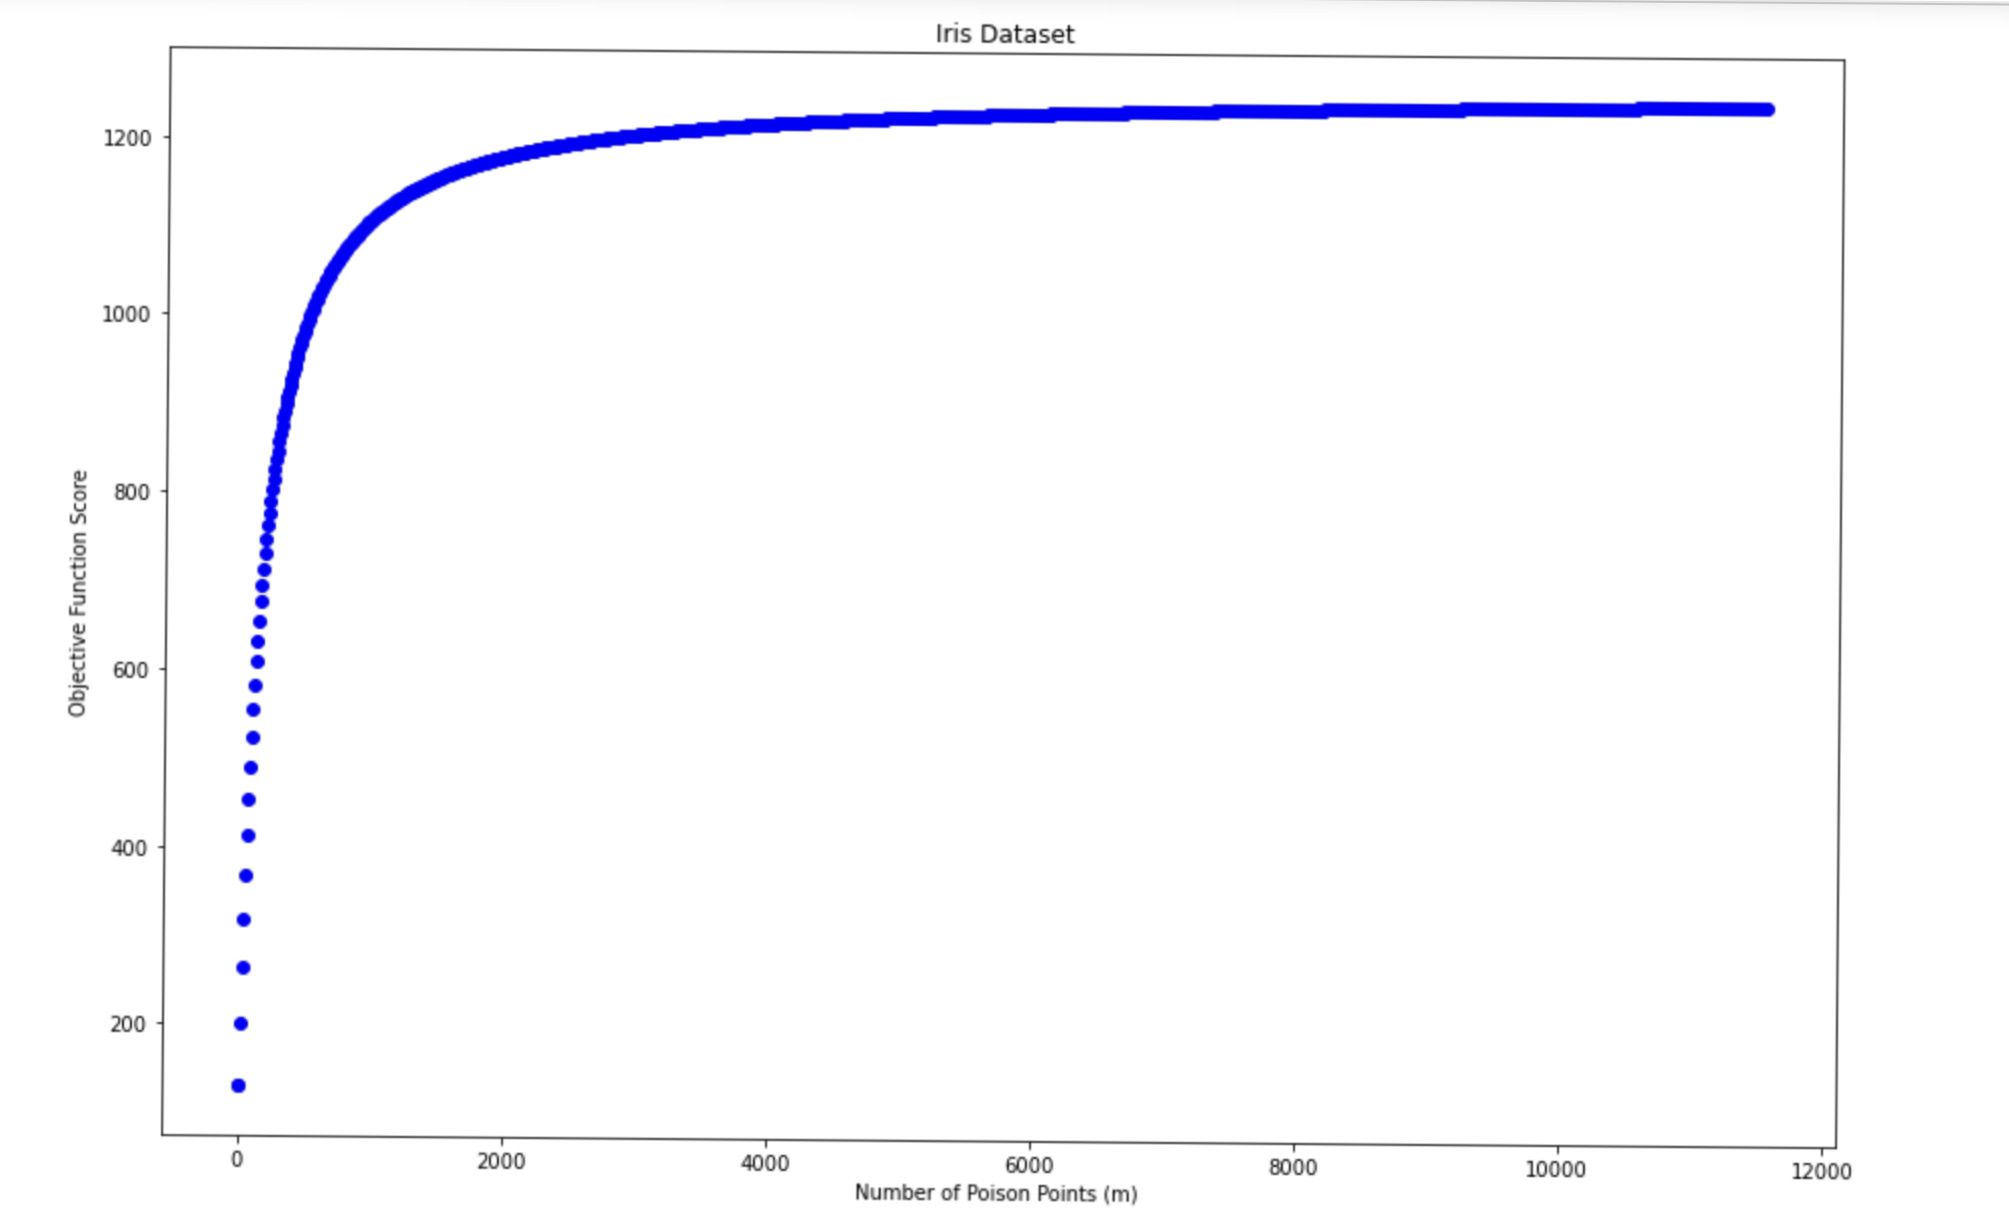
\includegraphics [width=5cm, height=4cm]{iris_poison_vs_score}

\section{Diabetes Data Experiment}
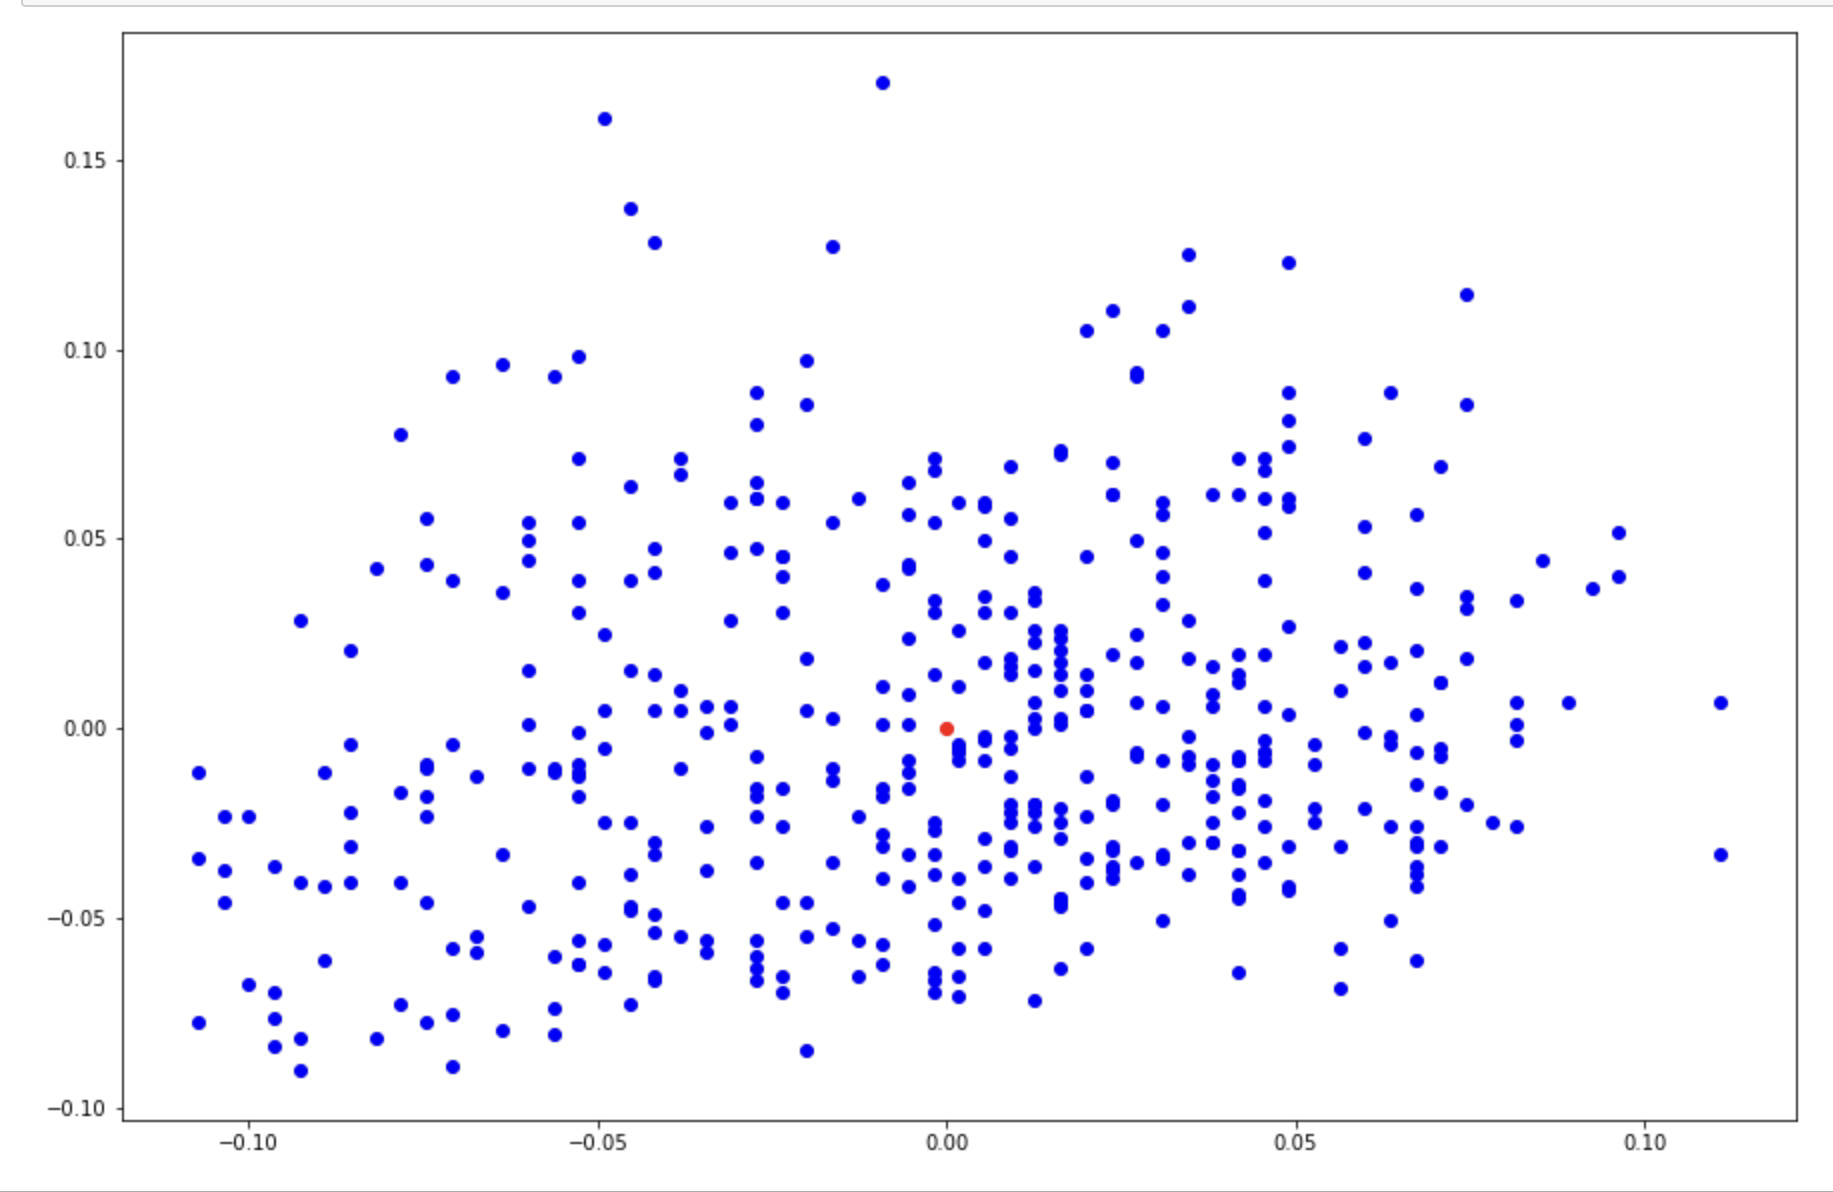
\includegraphics [width=5cm, height=4cm]{diabetes_data}
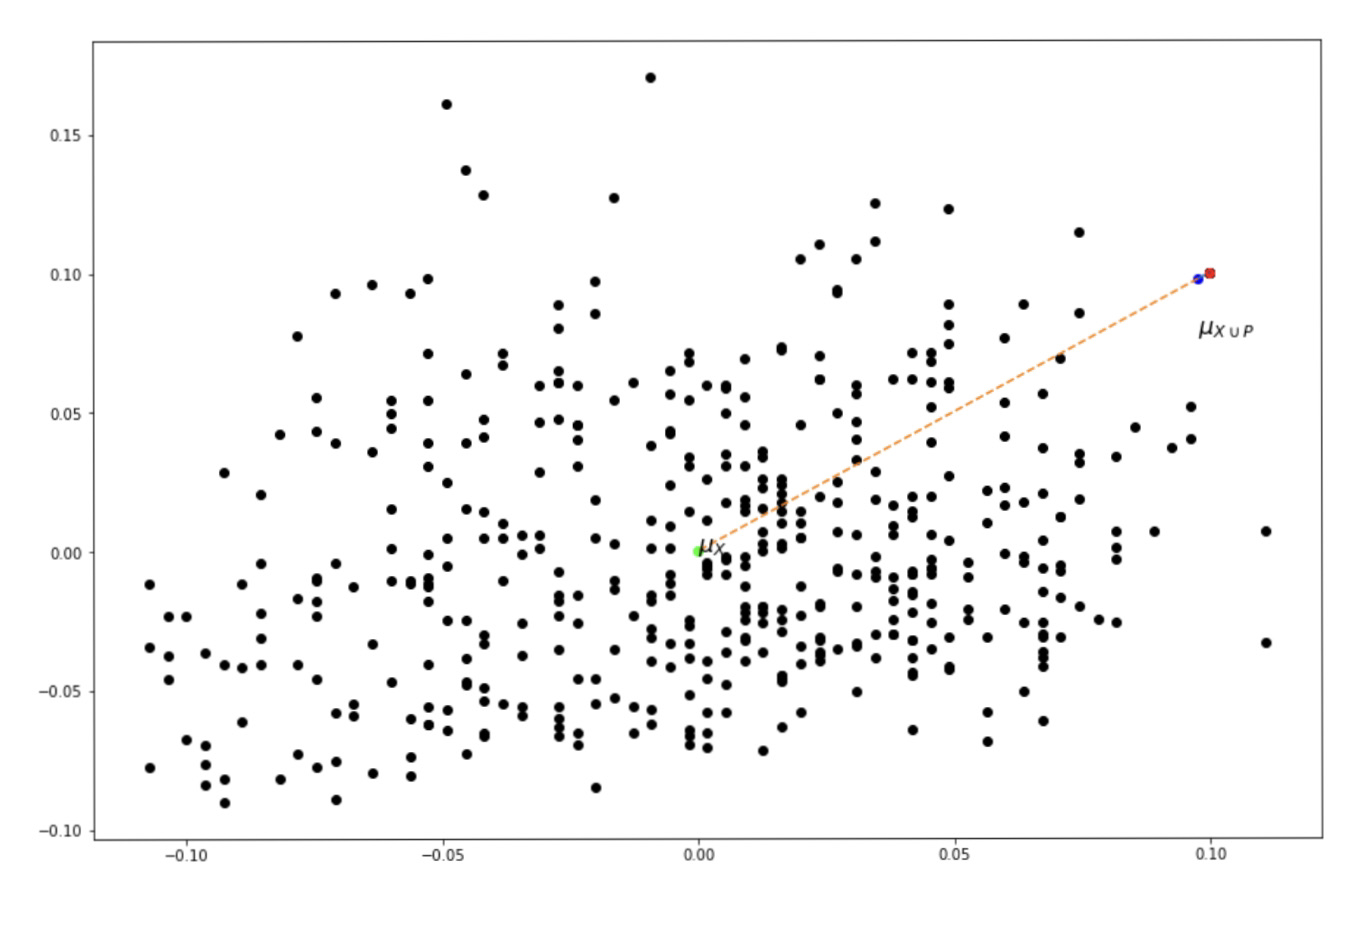
\includegraphics [width=5cm, height=4cm]{diabetes_data_poisoned}
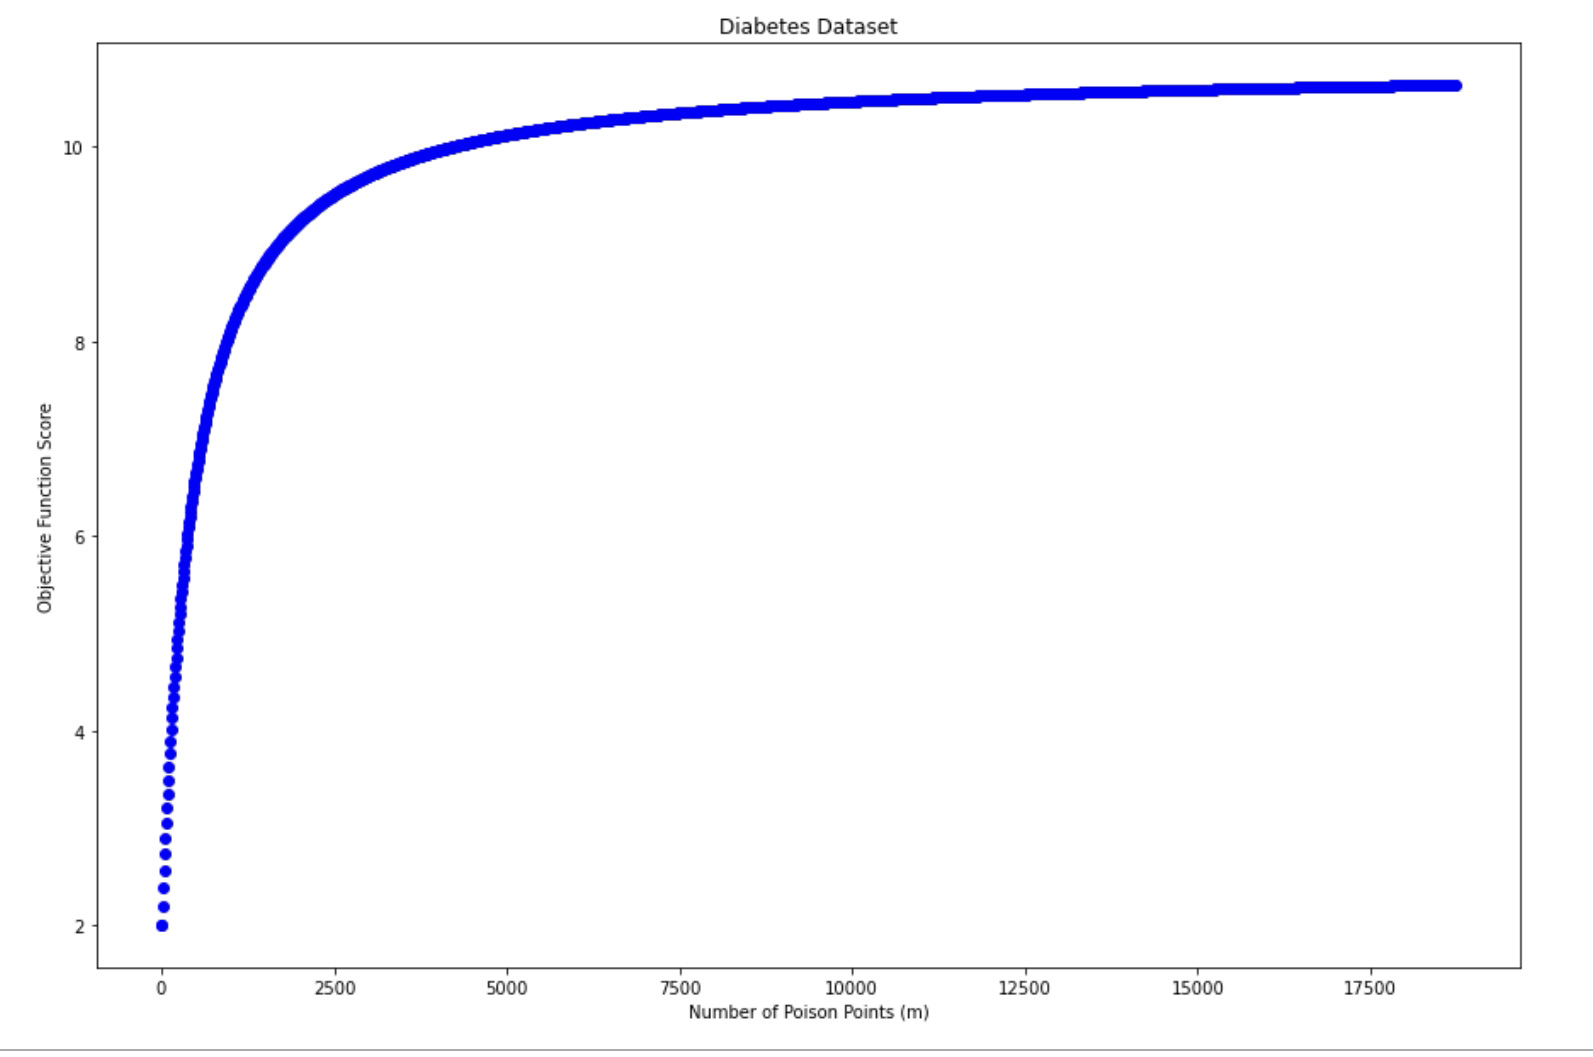
\includegraphics [width=5cm, height=4cm]{diabetes_poison_vs_score}


\end{document}

\end{document}